\documentclass[journal]{IEEEtran}
\usepackage[a5paper, margin=10mm]{geometry}
%\usepackage{lmodern} % Ensure lmodern is loaded for pdflatex
\usepackage{tfrupee} % Include tfrupee package


\setlength{\headheight}{1cm} % Set the height of the header box
\setlength{\headsep}{0mm}     % Set the distance between the header box and the top of the text


%\usepackage[a5paper, top=10mm, bottom=10mm, left=10mm, right=10mm]{geometry}

%
\setlength{\intextsep}{10pt} % Space between text and floats

\makeindex


\usepackage{cite}
\usepackage{amsmath,amssymb,amsfonts,amsthm}
\usepackage{algorithmic}
\usepackage{graphicx}
\usepackage{textcomp}
\usepackage{xcolor}
\usepackage{txfonts}
\usepackage{listings}
\usepackage{enumitem}
\usepackage{mathtools}
\usepackage{gensymb}
\usepackage{comment}
\usepackage[breaklinks=true]{hyperref}
\usepackage{tkz-euclide} 
\usepackage{listings}
\usepackage{multicol}
\usepackage{xparse}
\usepackage{gvv}
%\def\inputGnumericTable{}                                 
\usepackage[latin1]{inputenc}                                
\usepackage{color}                                            
\usepackage{array}                                            
\usepackage{longtable}                                       
\usepackage{calc}                                             
\usepackage{multirow}                                         
\usepackage{hhline}                                           
\usepackage{ifthen}                                               
\usepackage{lscape}
\usepackage{tabularx}
\usepackage{array}
\usepackage{float}
\usepackage{ar}
\usepackage[version=4]{mhchem}


\newtheorem{theorem}{Theorem}[section]
\newtheorem{problem}{Problem}
\newtheorem{proposition}{Proposition}[section]
\newtheorem{lemma}{Lemma}[section]
\newtheorem{corollary}[theorem]{Corollary}
\newtheorem{example}{Example}[section]
\newtheorem{definition}[problem]{Definition}
\newcommand{\BEQA}{\begin{eqnarray}}
\newcommand{\EEQA}{\end{eqnarray}}

\theoremstyle{remark}


\begin{document}
\bibliographystyle{IEEEtran}
\onecolumn

\title{10.4.3}
\author{INDHIRESH S- EE25BTECH11027}
\maketitle


\renewcommand{\thefigure}{\theenumi}
\renewcommand{\thetable}{\theenumi}

\textbf{Question}.The point at which the normal to the curve
$y = x +\frac{1}{x}$, $x > 0$ is perpendicular to the line $3x - 4y - 7 = 0$

\textbf{Solution}:\\
Let us solve the given equation theoretically and then verify the solution computationally. \\
The given curve be rearranged as:
\begin{align}
x^2-xy+1=0.
\end{align}
This can be expressed in the form:
\begin{align}
\Vec{x}^T\Vec{V}\Vec{x}+2\Vec{u}^T\vec{x}+f=0
\end{align}
Where:
\begin{align}
\Vec{v}=\myvec{1&-\frac{1}{2}\\-\frac{1}{2}&0}\;\;,\Vec{u}=\myvec{0\\0}\;\;and\;\;f=1
\end{align}
The required direction of normal which is perpendicular to the line $3x-4y-7=0$
\begin{align}
\Vec{m}=\myvec{1\\-\frac{4}{3}}
\end{align}

\begin{align}
 \Vec{m}=\myvec{3\\-4}
\end{align}
Now the equation of normal to the conic at the point of contact $\Vec{q}$ is given by:
\begin{align}
   (\Vec{V}\Vec{q}+\Vec{u})^T\Vec{R}(\Vec{x}-\Vec{q})=0
\end{align}
In the normal equation $\Vec{V}\Vec{q}+\Vec{u}$ is proportional to the direction vector of the normal.So,
\begin{align}
 \Vec{V}\Vec{q}+\Vec{u}=k\Vec{m}
\end{align}
\begin{align}
 \Vec{q}=\Vec{V}^{-1}(k\Vec{m}-\Vec{u})
\end{align}
$\Vec{q}$ lies on the curve.So substituting Eq.8 in Eq.2:
\begin{align}
    (\Vec{V}^{-1}(k\Vec{m}-\Vec{u}))^T\Vec{V}\Vec{V}^{-1}(k\Vec{m}-\Vec{u})+2\Vec{u}^T\Vec{V}^{-1}(k\Vec{m}-\Vec{u})+f=0
\end{align}
\begin{align}
    (\Vec{V}^{-1}(k\Vec{m}-\Vec{u}))^T(k\Vec{m}-\Vec{u})+f=0
\end{align}
\begin{align}
    \brak{\myvec{0&-2\\-2&-4}\myvec{k\myvec{3\\-4}-\myvec{0\\0}}}^T\myvec{k\myvec{3\\-4}-\myvec{0\\0}} +1=0
\end{align}
\begin{align}
     k^2\myvec{3&-4}\myvec{0&-2\\-2&-4}\myvec{3\\-4}+1=0
\end{align}
\begin{align}
    k^2=\frac{1}{16}
\end{align}
\begin{align}
    k=\frac{1}{4}\;\;and\;\;k=-\frac{1}{4}
\end{align}
Now substitute the corresponding values in the Eq.8 to get the point
\begin{align}
    \Vec{q}=\myvec{0&-2\\-2&-4}\myvec{k\myvec{3\\-4}-\myvec{0\\0}}
\end{align}
\begin{align}
    \Vec{q}=k\myvec{0&-2\\-2&-4}\myvec{3\\-4}
\end{align}
\begin{align}
    \Vec{q}=k\myvec{8\\10}
\end{align}
When $k=\frac{1}{4}$
\begin{align}
    \Vec{q}=\myvec{2\\\frac{5}{2}}
\end{align}
When $k=-\frac{1}{4}$
\begin{align}
    \Vec{q}=\myvec{-2\\-\frac{5}{2}}
\end{align}
Given that $x>0$ . So the point of contact is 
\begin{align}
     \Vec{q}=\myvec{2\\\frac{5}{2}}
\end{align}
From the figure it is clearly verified that the theoretical solution matches with the computational solution.\\
\begin{figure}[h]
    \centering
    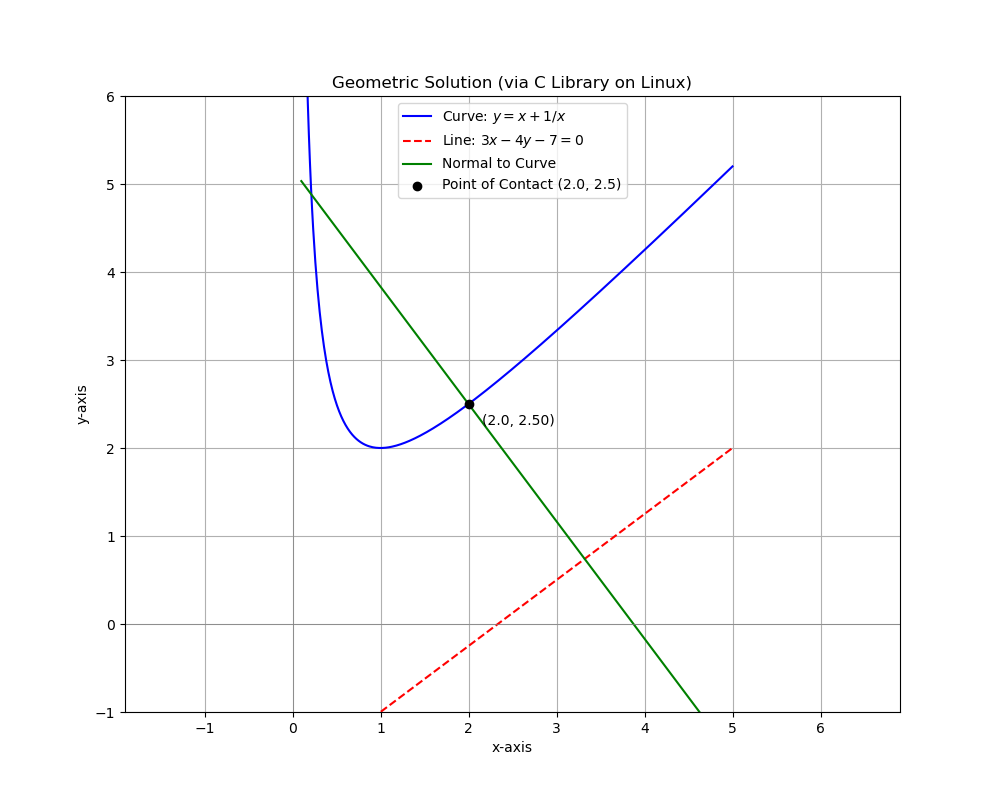
\includegraphics[height=0.5\textheight, keepaspectratio]{figs/figure1.png}
    \label{figure_1}
\end{figure}

\end{document}